\documentclass[11pt,a4paper]{article}
\usepackage[utf8]{inputenc}
\usepackage{graphicx}
\usepackage{multirow}
\usepackage{enumitem}
\usepackage{amsmath,amssymb}
\usepackage{array}
\usepackage{tikz}
\usetikzlibrary{decorations.pathmorphing,arrows.meta}
\usepackage[left=10mm,right=20mm,top=20mm,bottom=10mm]{geometry}

\newcommand{\xx}{\mathbf{x}}
\graphicspath{{C:/Users/teoso/Documents/Template Math Depart/}}
\setlist[enumerate,1]{label=\arabic*.,leftmargin=*,itemsep=10pt,parsep=0pt,topsep=6pt}
\setlist[enumerate,2]{label=(\alph*),leftmargin=*,itemsep=7pt,parsep=0pt,topsep=5pt}

\begin{document}
\pagenumbering{gobble}
\setlength{\abovedisplayskip}{7pt}
\setlength{\belowdisplayskip}{7pt}
\setlength{\abovedisplayshortskip}{4pt}
\setlength{\belowdisplayshortskip}{4pt}

\noindent
\begin{minipage}{0.15\textwidth}
  \includegraphics[width=1.8cm]{ITS.png}
\end{minipage}%
\begin{minipage}{0.7\textwidth}
  \centering
  \textbf{EVALUASI TENGAH SEMESTER GASAL 2025/2026}\\
  \textbf{DEPARTEMEN MATEMATIKA FSAD ITS}\\
  \textbf{PROGRAM SARJANA}
\end{minipage}%
\begin{minipage}{0.15\textwidth}
  \centering
  \includegraphics[width=1.8cm]{M.png}
\end{minipage}

\vspace{0.4cm}
\noindent
\begin{tabular}{@{}l c l@{}}
  Mata Kuliah  & : & Matematika Sistem\\
  Hari/Tanggal & : & Kamis, 16 Oktober 2025\\
  Waktu/Sifat  & : & 100 Menit / Tertutup\\
  Dosen        & : & Prof. Dr. Mardlijah, M.T.\\
               &   & Dr. Tahiyatul Asfihani, S.Si., M.Si.\\
               &   & Dr. Didik K.A., S.Si., M.Si.\\
               &   & Prof. Subchan, M.Sc., Ph.D.
\end{tabular}

\vspace{0.3cm}
\noindent\fbox{\parbox{\dimexpr\textwidth-2\fboxsep-2\fboxrule\relax}{%
  \textbf{HARAP DIPERHATIKAN !!!}\\
  Segala jenis pelanggaran (mencontek, kerjasama, dsb) yang dilakukan saat ETS/EAS
  akan dikenakan sanksi pembatalan mata kuliah pada semester yang sedang berjalan.
}}

\vspace{0.3cm}
\noindent ETS mengukur kemampuan
\begin{center}
  \begin{tabular}{|>{\centering\arraybackslash}p{1.6cm}|>{\raggedright\arraybackslash}p{\dimexpr\textwidth-6.2cm-14\tabcolsep-8\arrayrulewidth\relax}|>{\centering\arraybackslash}p{2cm}|>{\centering\arraybackslash}p{0.65cm}|>{\centering\arraybackslash}p{0.65cm}|>{\centering\arraybackslash}p{0.65cm}|>{\centering\arraybackslash}p{0.65cm}|}
    \hline
    \multicolumn{2}{|c|}{CPMK}
      & \multirow{2}{*}{\shortstack{Bobot\\CPMK (\%)}}
      & \multicolumn{4}{c|}{CPL}\\ \cline{4-7}
    \multicolumn{2}{|c|}{} & & 5 & 6 & 8 & 9\\ \hline
    CPMK-1 & Mampu mengidentifikasi fenomena alam, masalah-masalah teknik dalam bentuk sistem
      & 12.5 & $\checkmark$ & $\checkmark$ & $\checkmark$ & $\checkmark$\\ \hline
    CPMK-2 & Mampu menganalisa sistem terutama sifat kestabilan, keterkontrolan dan keteramatannya serta mampu menyusun input pengendali sistem
      & 12.5 & $\checkmark$ & $\checkmark$ & $\checkmark$ & $\checkmark$\\ \hline
  \end{tabular}
\end{center}

\begin{center}
  \renewcommand{\arraystretch}{1.65}
  \begin{tabular}{|c|p{10.5cm}|c|c|}
    \hline
    \multicolumn{2}{|c|}{CPMK} & Soal & Skor\\ \hline
    \multirow{2}{*}{CPMK-1}
      & \multirow{2}{10.5cm}{Mampu mengidentifikasi fenomena alam, masalah-masalah teknik dalam bentuk sistem}
      & 1 & 25\\ \cline{3-4}
      & & 2 & 25\\ \hline
    \multirow{2}{*}{CPMK-2}
      & \multirow{2}{10.5cm}{Mampu menganalisa sistem terutama sifat kestabilan, keterkontrolan dan keteramatannya serta mampu menyusun input pengendali sistem}
      & 3 & 25\\ \cline{3-4}
      & & 4 & 25\\ \hline
  \end{tabular}
\end{center}

\begin{center}
  Soal
\end{center}
\begin{enumerate}
  \item Diberikan sistem rangkaian listrik sebagai berikut:
        \begin{center}
          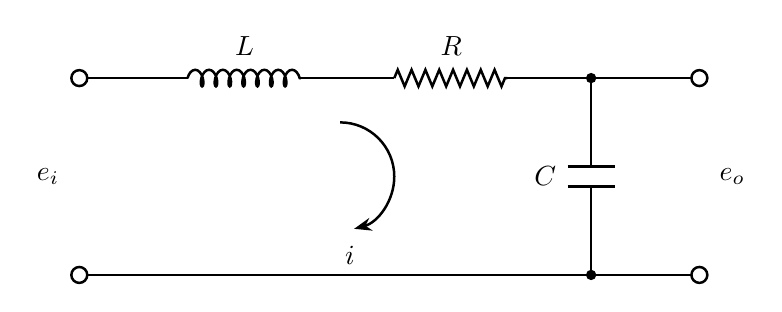
\begin{tikzpicture}[scale=1.25,line width=0.9pt]
            \draw (0,2) -- (1.1,2);
            \draw[decorate,decoration={coil,aspect=0.5,segment length=5pt,amplitude=3pt}]
              (1.1,2) -- (2.25,2);
            \draw (2.25,2) -- (3.2,2);
            \draw[decorate,decoration={zigzag,segment length=5pt,amplitude=3pt}]
              (3.2,2) -- (4.35,2);
            \draw (4.35,2) -- (6.3,2);
            \draw (0,0) -- (6.3,0);
            \draw (5.2,2) -- (5.2,1.1);
            \draw (4.96,1.1) -- (5.44,1.1);
            \draw (4.96,0.9) -- (5.44,0.9);
            \draw (5.2,0.9) -- (5.2,0);
            \fill (5.2,2) circle (1.5pt);
            \fill (5.2,0) circle (1.5pt);
            \foreach \p in {(0,2),(0,0),(6.3,2),(6.3,0)}
              \draw[fill=white] \p circle (2.3pt);
            \node[above] at (1.68,2.12) {$L$};
            \node[above] at (3.78,2.12) {$R$};
            \node[left] at (4.95,1) {$C$};
            \node[left] at (-0.1,1) {$e_i$};
            \node[right] at (6.4,1) {$e_o$};
            \draw[-{Stealth[length=2.2mm]}] (2.65,1.55)
              arc[start angle=90,end angle=-75,radius=0.55];
            \node[below] at (2.75,0.4) {$i$};
          \end{tikzpicture}
        \end{center}

        \vfill
        \begin{center}
          \textit{Selamat Mengerjakan}
        \end{center}
        \newpage

        Persamaan diferensial dari sistem tersebut adalah
        \[
          e_0''+\frac{R}{L}e_0'+\frac{1}{LC}e_0=\frac{1}{LC}e_1.
        \]
        Dengan mendefinisikan variabel state $x_1=e_0$, $x_2=e_0'$,
        ubahlah persamaan diferensial tersebut dalam bentuk state space.
        Diketahui $e_1$ adalah input sistem dan
        \begin{enumerate}
          \item keluaran sistem adalah $x_2$;
          \item keluaran sistem adalah $x_1$ dan $x_2$.
        \end{enumerate}

  \item Diberikan sistem berikut:
        \[
          \begin{aligned}
            \dot{x}(t)&=x(t)-x(t)^2-x(t)y(t),\\
            \dot{y}(t)&=2y(t)-0.5y(t)^2-x(t)y(t).
          \end{aligned}
        \]
        \begin{enumerate}
          \item Linearkan sistem tersebut di sekitar penyelesaian $x(t)=y(t)=0$.
          \item Dapatkan penyelesaian sistem linier dari hasil pelinieran (a)
                bila diberikan $x(0)=1$ dan $y(0)=3$.
        \end{enumerate}

  \item Diberikan sistem dinamik
        \[
          \dot{\xx}(t)=A\xx(t)+Bu(t)
        \]
        dan output
        \[
          y(t)=C\xx(t),
        \]
        dengan
        \[
          A=\begin{bmatrix}3&-2\\-1&2\end{bmatrix},\qquad
          B=\begin{bmatrix}1\\0\end{bmatrix},\qquad
          C=\begin{bmatrix}0&1\end{bmatrix},\qquad u(t)=e^{-t}.
        \]
        \begin{enumerate}
          \item Tentukan matriks fundamental dan matriks transisi dari sistem tersebut.
          \item Tentukan $e^{At}$.
          \item Tuliskan penyelesaian $\xx(t)$ dan output $y(t)$ dalam bentuk matriks transisi
                yang diperoleh dari poin (a) dan (b).
        \end{enumerate}

  \item Pandang sistem yang berbentuk
        \[
          \dot{\xx}(t)=
          \begin{bmatrix}4&0&0\\0&-2&5\\0&2&1\end{bmatrix}\xx(t)
          +\begin{bmatrix}0\\1\\0\end{bmatrix}u(t),
          \qquad
          y(t)=\begin{bmatrix}1&0&0\end{bmatrix}\xx(t).
        \]
        \begin{enumerate}
          \item Lakukan analisa kestabilan dengan menggunakan kriteria Routh--Hurwitz terhadap sistem tersebut.
          \item Carilah eigen value dari sistem tersebut.
                Apakah sesuai dengan kestabilan yang diperoleh pada soal (a)?
        \end{enumerate}
\end{enumerate}

\vfill
\begin{center}
  \textit{Selamat mengerjakan, semoga sukses.}\\
  \textit{Kejujuran adalah modal utama suatu keberhasilan.}
\end{center}
\newpage

\begin{center}
  Solusi
\end{center}
\begin{enumerate}[itemsep=12pt,parsep=5pt]
  \item Gunakan $u(t)=e_1(t)$ sebagai input.
        Ini adalah tegangan masukan $e_i$ pada gambar.
        Definisikan vektor state $\xx=(x_1,x_2)^{\mathsf T}$.
        Dari $x_1=e_0$ dan $x_2=e_0'$, diperoleh
        \[
          \dot{x}_1=x_2.
        \]
        Susun kembali persamaan diferensial untuk memperoleh turunan kedua:
        \[
          \dot{x}_2=e_0''
          =-\frac{1}{LC}x_1-\frac{R}{L}x_2+\frac{1}{LC}u.
        \]
        Jadi, persamaan state-nya adalah
        \[
          \dot{\xx}=A\xx+Bu,\qquad
          A=\begin{bmatrix}0&1\\-\dfrac{1}{LC}&-\dfrac{R}{L}\end{bmatrix},
          \qquad B=\begin{bmatrix}0\\\dfrac{1}{LC}\end{bmatrix}.
        \]
        Matriks $A$ dan $B$ berlaku untuk kedua pilihan keluaran.
        \begin{enumerate}
          \item Jika keluarannya $x_2$, maka
                \[
                  y=x_2=C_a\xx+D_a u,\qquad
                  C_a=\begin{bmatrix}0&1\end{bmatrix},\qquad D_a=0.
                \]
                Keluaran diperoleh dengan mengambil komponen kedua vektor state.

          \item Jika keluarannya $x_1$ dan $x_2$, bentuk vektor keluaran
                \[
                  \mathbf{y}=\begin{bmatrix}x_1\\x_2\end{bmatrix}
                  =C_b\xx+D_bu.
                \]
                Karena kedua komponen state menjadi keluaran,
                \[
                  C_b=\begin{bmatrix}1&0\\0&1\end{bmatrix},\qquad
                  D_b=\begin{bmatrix}0\\0\end{bmatrix}.
                \]
        \end{enumerate}

  \item Tuliskan ruas kanan sebagai
        \[
          f(x,y)=x-x^2-xy,\qquad g(x,y)=2y-\frac12y^2-xy.
        \]
        Karena $f(0,0)=g(0,0)=0$, titik $(0,0)$ merupakan titik setimbang.
        \begin{enumerate}
          \item Pelinieran diperoleh dari matriks Jacobian di titik setimbang.
                Turunan parsialnya memberikan
                \[
                  J(x,y)=\begin{bmatrix}
                    \dfrac{\partial f}{\partial x}&\dfrac{\partial f}{\partial y}\\[5pt]
                    \dfrac{\partial g}{\partial x}&\dfrac{\partial g}{\partial y}
                  \end{bmatrix}
                  =\begin{bmatrix}1-2x-y&-x\\-y&2-y-x\end{bmatrix}.
                \]
                Substitusikan $x=y=0$:
                \[
                  J(0,0)=\begin{bmatrix}1&0\\0&2\end{bmatrix}.
                \]
                Misalkan $x_{\ell},y_{\ell}$ menyatakan variabel pada model linier.
                Karena titik setimbangnya nol, sistem hasil pelinierannya adalah
                \[
                  \begin{bmatrix}\dot{x}_{\ell}\\\dot{y}_{\ell}\end{bmatrix}
                  =\begin{bmatrix}1&0\\0&2\end{bmatrix}
                   \begin{bmatrix}x_{\ell}\\y_{\ell}\end{bmatrix}.
                \]

          \item Kedua persamaan linier tersebut saling terpisah:
                \[
                  \dot{x}_{\ell}=x_{\ell},\qquad \dot{y}_{\ell}=2y_{\ell}.
                \]
                Solusi umumnya adalah $x_{\ell}(t)=k_1e^t$ dan $y_{\ell}(t)=k_2e^{2t}$.
                Syarat awal $x_{\ell}(0)=1$ memberikan $k_1=1$.
                Syarat awal $y_{\ell}(0)=3$ memberikan $k_2=3$.
                Jadi, solusi model liniernya adalah
                \[
                  x_{\ell}(t)=e^t,\qquad y_{\ell}(t)=3e^{2t}.
                \]
        \end{enumerate}

  \item Matriks fundamental dibentuk dari solusi homogen yang bebas linier.
        Matriks transisi memetakan state pada waktu awal ke state pada waktu berikutnya untuk sistem homogen.
        \begin{enumerate}
          \item Untuk sistem homogen $\dot{\xx}=A\xx$, tentukan nilai eigen $A$:
                \begin{align*}
                  \det(A-\lambda I)
                    &=(3-\lambda)(2-\lambda)-2\\
                    &=\lambda^2-5\lambda+4\\
                    &=(\lambda-1)(\lambda-4).
                \end{align*}
                Jadi, nilai eigennya $\lambda_1=1$ dan $\lambda_2=4$.

                Untuk $\lambda_1=1$, persamaan $(A-I)v=0$ memberikan $v_1=v_2$.
                Pilih vektor eigen $p_1=(1,1)^{\mathsf T}$.
                Untuk $\lambda_2=4$, persamaan $(A-4I)v=0$ memberikan $v_1=-2v_2$.
                Pilih $p_2=(-2,1)^{\mathsf T}$.
                Maka,
                \[
                  P=\begin{bmatrix}1&-2\\1&1\end{bmatrix},\qquad
                  P^{-1}=\frac13\begin{bmatrix}1&2\\-1&1\end{bmatrix}.
                \]
                Setiap fungsi $e^{\lambda t}p$ memenuhi persamaan homogen jika $Ap=\lambda p$.
                Jadi, salah satu matriks fundamentalnya adalah
                \[
                  F(t)=\begin{bmatrix}e^t&-2e^{4t}\\e^t&e^{4t}\end{bmatrix}
                      =P\begin{bmatrix}e^t&0\\0&e^{4t}\end{bmatrix}.
                \]
                Kolom-kolomnya bebas linier karena $\det F(t)=3e^{5t}\ne0$.

                Untuk waktu awal $t_0$, matriks transisinya adalah
                \begin{align*}
                  \Phi(t,t_0)
                    &=F(t)F(t_0)^{-1}\\
                    &=P\begin{bmatrix}e^{t-t_0}&0\\0&e^{4(t-t_0)}\end{bmatrix}P^{-1}.
                \end{align*}
                Tuliskan $\Delta=t-t_0$.
                Setelah perkalian matriks, diperoleh
                \[
                  \Phi(t,t_0)=\frac13\begin{bmatrix}
                    e^{\Delta}+2e^{4\Delta}&2e^{\Delta}-2e^{4\Delta}\\
                    e^{\Delta}-e^{4\Delta}&2e^{\Delta}+e^{4\Delta}
                  \end{bmatrix}.
                \]
                Untuk $t=t_0$, berlaku $\Phi(t_0,t_0)=I$.

          \item Karena $A$ konstan, $e^{At}=\Phi(t,0)$.
                Substitusikan $t_0=0$ pada hasil (a):
                \[
                  e^{At}=\frac13\begin{bmatrix}
                    e^t+2e^{4t}&2e^t-2e^{4t}\\
                    e^t-e^{4t}&2e^t+e^{4t}
                  \end{bmatrix}.
                \]
                Hasil ini memenuhi $e^{A\cdot0}=I$.

          \item Nyatakan kondisi awal sebagai $\xx(0)=\xx_0=(\alpha,\beta)^{\mathsf T}$.
                Rumus penyelesaian sistem dengan input adalah
                \[
                  \xx(t)=\Phi(t,0)\xx_0+\int_0^t\Phi(t,\tau)Bu(\tau)\,d\tau.
                \]
                Dengan $B=(1,0)^{\mathsf T}$ dan $u(\tau)=e^{-\tau}$,
                \[
                  \Phi(t,\tau)Bu(\tau)
                  =\frac13\begin{bmatrix}
                    e^{t-\tau}+2e^{4(t-\tau)}\\
                    e^{t-\tau}-e^{4(t-\tau)}
                  \end{bmatrix}e^{-\tau}.
                \]
                Misalkan kontribusi input tersebut adalah $q(t)$.
                Pisahkan integral pada kedua komponennya:
                \[
                  q(t)=\frac13\begin{bmatrix}
                    e^t\displaystyle\int_0^t e^{-2\tau}\,d\tau
                      +2e^{4t}\displaystyle\int_0^t e^{-5\tau}\,d\tau\\[8pt]
                    e^t\displaystyle\int_0^t e^{-2\tau}\,d\tau
                      -e^{4t}\displaystyle\int_0^t e^{-5\tau}\,d\tau
                  \end{bmatrix}.
                \]
                Kedua integralnya adalah
                \[
                  \int_0^t e^{-2\tau}\,d\tau=\frac{1-e^{-2t}}2,\qquad
                  \int_0^t e^{-5\tau}\,d\tau=\frac{1-e^{-5t}}5.
                \]
                Substitusikan dan sederhanakan:
                \[
                  q(t)=\frac1{30}\begin{bmatrix}
                    5e^t+4e^{4t}-9e^{-t}\\
                    5e^t-2e^{4t}-3e^{-t}
                  \end{bmatrix}.
                \]
                Jadi, penyelesaian state-nya adalah
                \[
                  \xx(t)=\Phi(t,0)\begin{bmatrix}\alpha\\\beta\end{bmatrix}
                  +\frac1{30}\begin{bmatrix}
                    5e^t+4e^{4t}-9e^{-t}\\
                    5e^t-2e^{4t}-3e^{-t}
                  \end{bmatrix}.
                \]
                Karena $C=\begin{bmatrix}0&1\end{bmatrix}$, output mengambil komponen kedua state:
                \[
                  y(t)=C\Phi(t,0)\xx_0
                       +\int_0^t C\Phi(t,\tau)Be^{-\tau}\,d\tau.
                \]
                Secara eksplisit,
                \[
                  y(t)=\frac{(e^t-e^{4t})\alpha+(2e^t+e^{4t})\beta}{3}
                      +\frac{5e^t-2e^{4t}-3e^{-t}}{30}.
                \]
        \end{enumerate}

  \item Untuk kestabilan internal, gunakan sistem homogen $\dot{\xx}=A\xx$.
        \begin{enumerate}
          \item Polinom karakteristiknya adalah
                \begin{align*}
                  p(s)=\det(sI-A)
                    &=(s-4)\begin{vmatrix}s+2&-5\\-2&s-1\end{vmatrix}\\
                    &=(s-4)\bigl((s+2)(s-1)-10\bigr)\\
                    &=(s-4)(s^2+s-12)\\
                    &=s^3-3s^2-16s+48.
                \end{align*}
                Dua baris pertama tabel Routh diambil dari koefisien polinom:
                \[
                  \begin{array}{c|rr}
                    s^3&1&-16\\
                    s^2&-3&48
                  \end{array}
                \]
                Entri pertama pada baris $s^1$ adalah
                \[
                  b_1=\frac{(-3)(-16)-(1)(48)}{-3}=0.
                \]
                Entri berikutnya juga nol.
                Jadi, seluruh baris $s^1$ bernilai nol.
                Gunakan polinom bantu dari baris $s^2$:
                \[
                  H(s)=-3s^2+48,\qquad H'(s)=-6s.
                \]
                Ganti baris nol dengan koefisien $H'(s)$, yaitu $(-6,0)$.
                Entri baris terakhir menjadi
                \[
                  c_1=\frac{(-6)(48)-(-3)(0)}{-6}=48.
                \]
                Tabel Routh lengkapnya adalah
                \[
                  \begin{array}{c|rr}
                    s^3&1&-16\\
                    s^2&-3&48\\
                    s^1&-6&0\\
                    s^0&48&0
                  \end{array}
                \]
                Kolom pertamanya memiliki urutan tanda $+,-,-,+$.
                Ada dua perubahan tanda.
                Maka, terdapat dua akar dengan bagian real positif.
                Jadi, sistem tidak stabil.

          \item Faktorkan polinom karakteristiknya:
                \[
                  p(\lambda)=(\lambda-4)(\lambda^2+\lambda-12)
                            =(\lambda-4)(\lambda+4)(\lambda-3).
                \]
                Jadi, nilai-nilai eigennya adalah
                \[
                  \lambda_1=4,\qquad\lambda_2=3,\qquad\lambda_3=-4.
                \]
                Ada dua nilai eigen positif.
                Hasil ini sesuai dengan ketidakstabilan pada tabel Routh.
        \end{enumerate}
\end{enumerate}

\end{document}
